\chapter{Сервис для анализа данных} \label{ch:ch4}

В этой главе будет рассмотрено устройство сервиса, которое было создано, чтобы упростить процесс анализа данных и поиска аномалий в них.

Ниже будут представлены основные сценарии работы с сервисом.

\section{Описание сервиса}

\begin{figure}[ht]
  \centering
  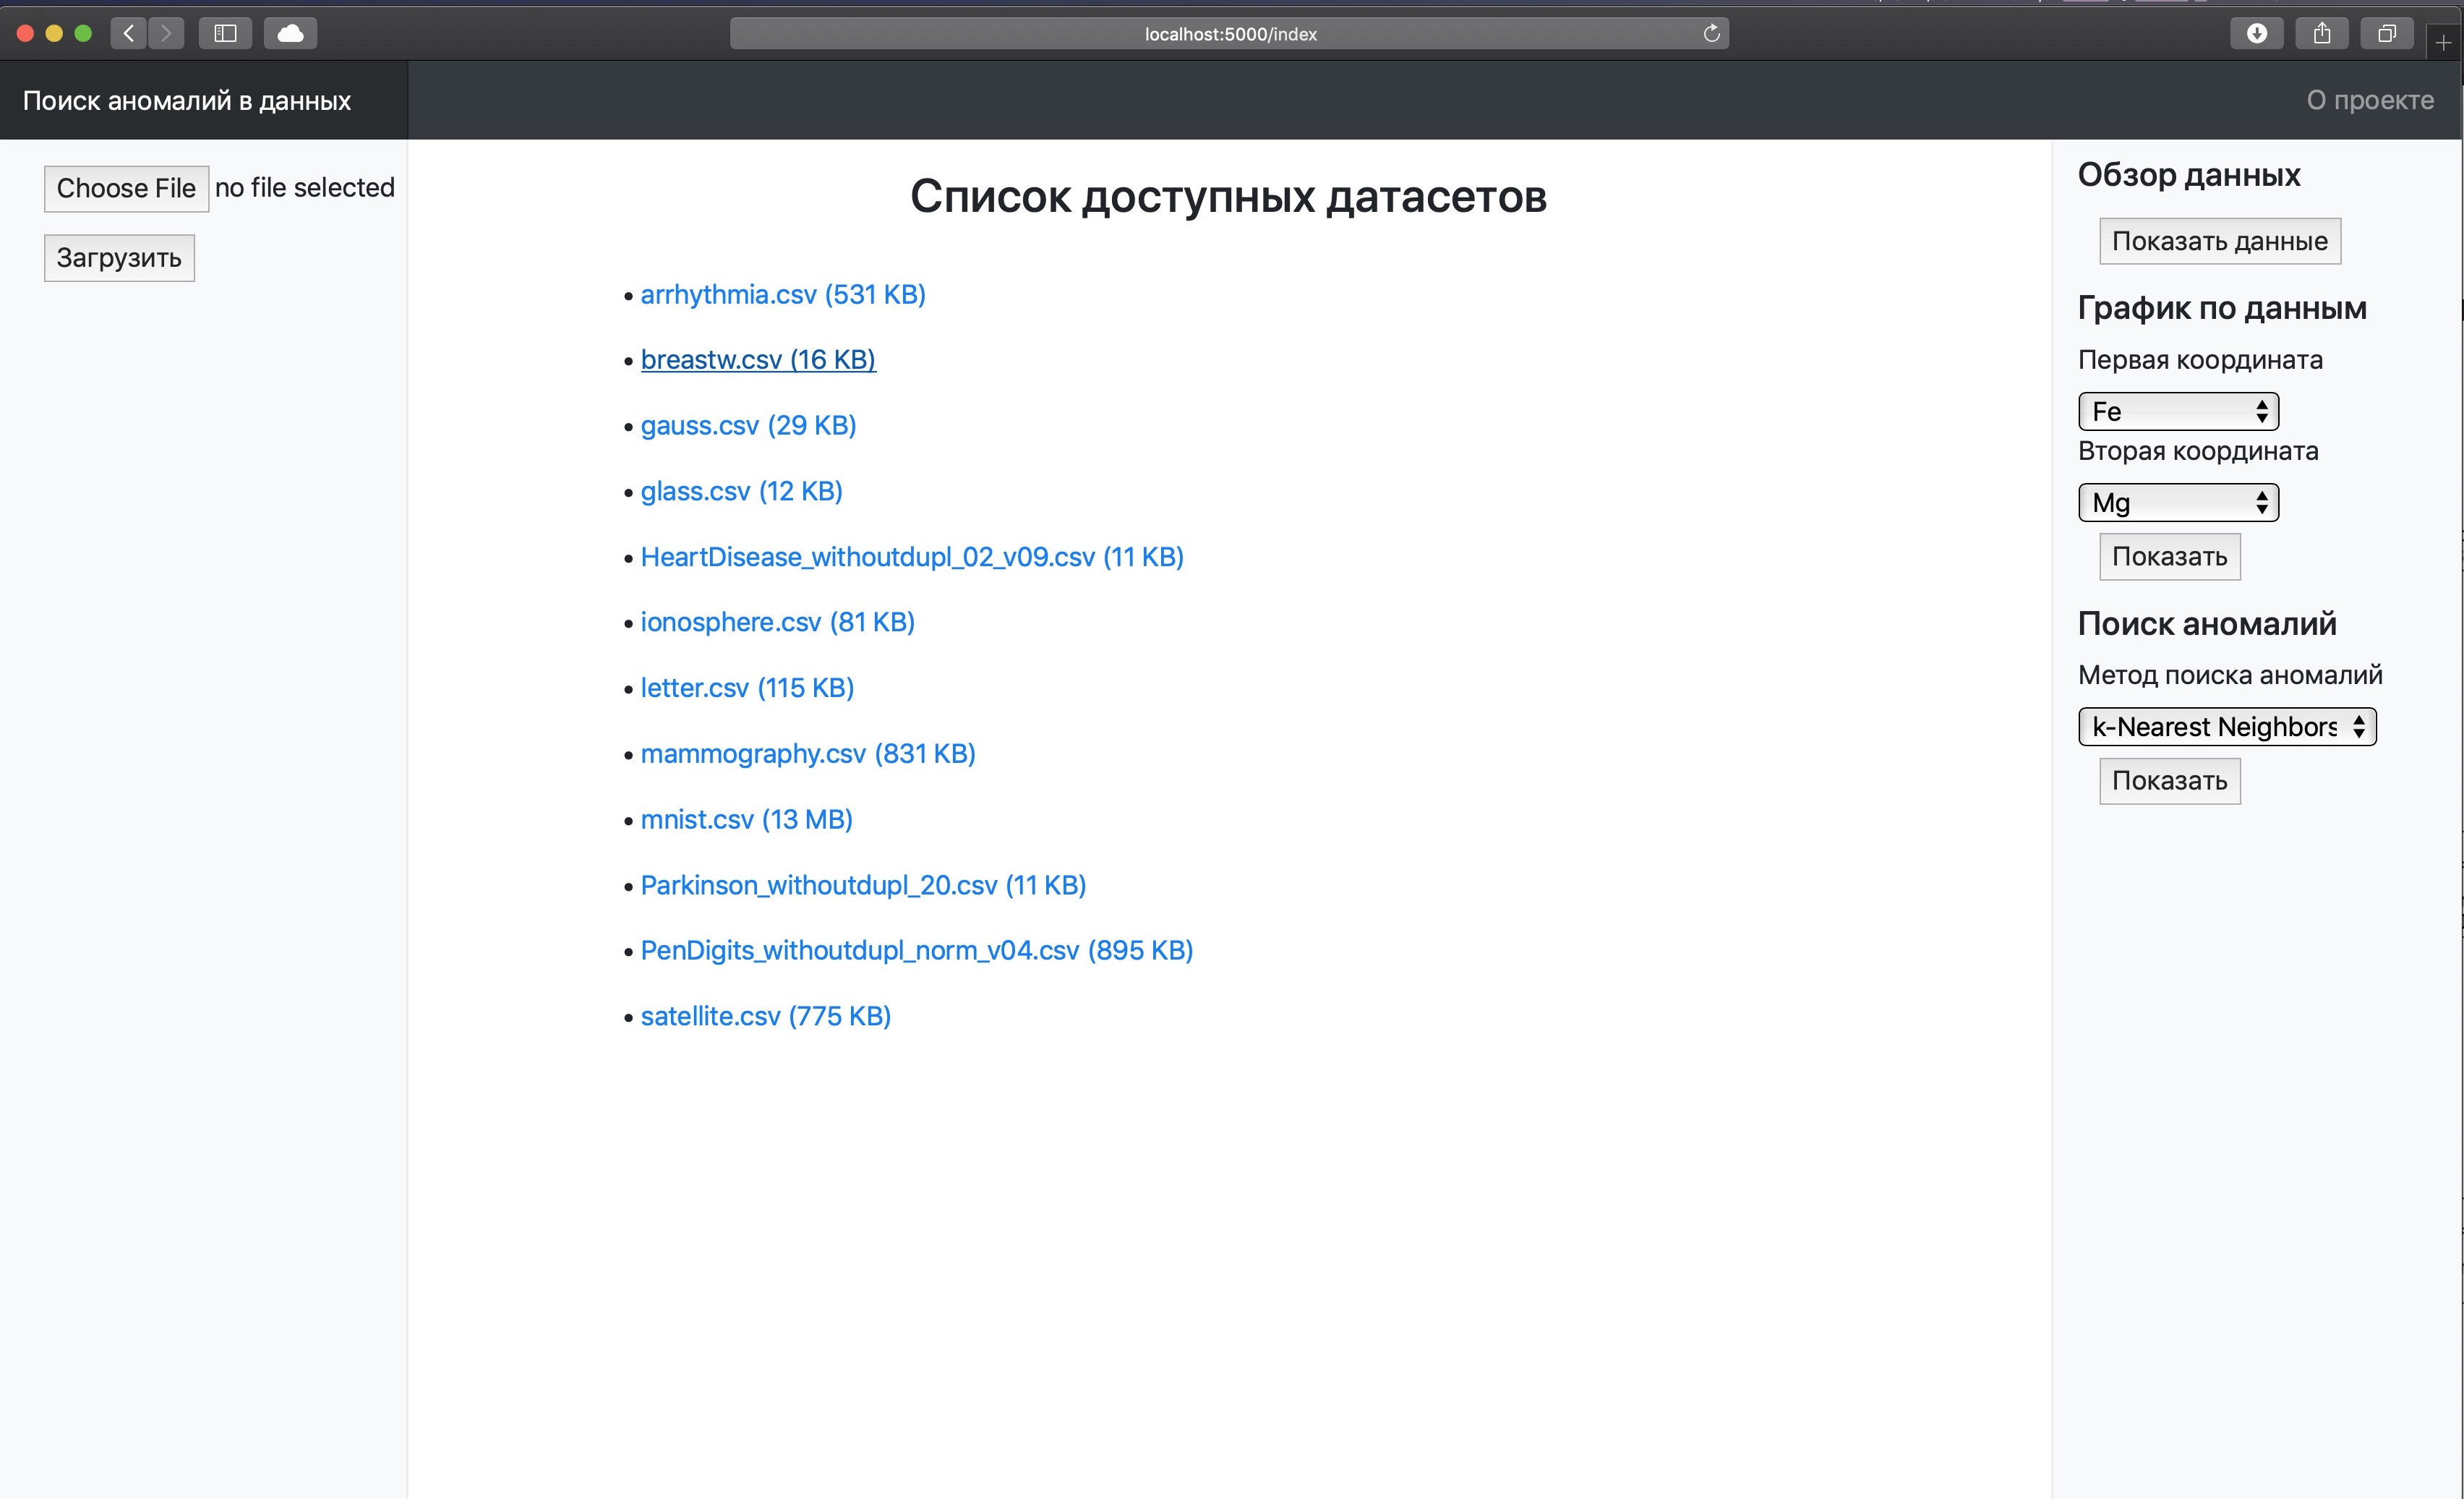
\includegraphics[width=\textwidth, height=\textheight, keepaspectratio] {demo_mainmenu}
  \caption{Главный экран сервиса. Есть возможность загрузить данные через окно загрузки (как продемонстрировано рисунке~\ref{fig:demo_uploadfile}), либо выбрать набор данных из списка загруженных ранее.}
  \label{fig:demo_mainmenu}
\end{figure}

\begin{figure}[ht]
  \centering
  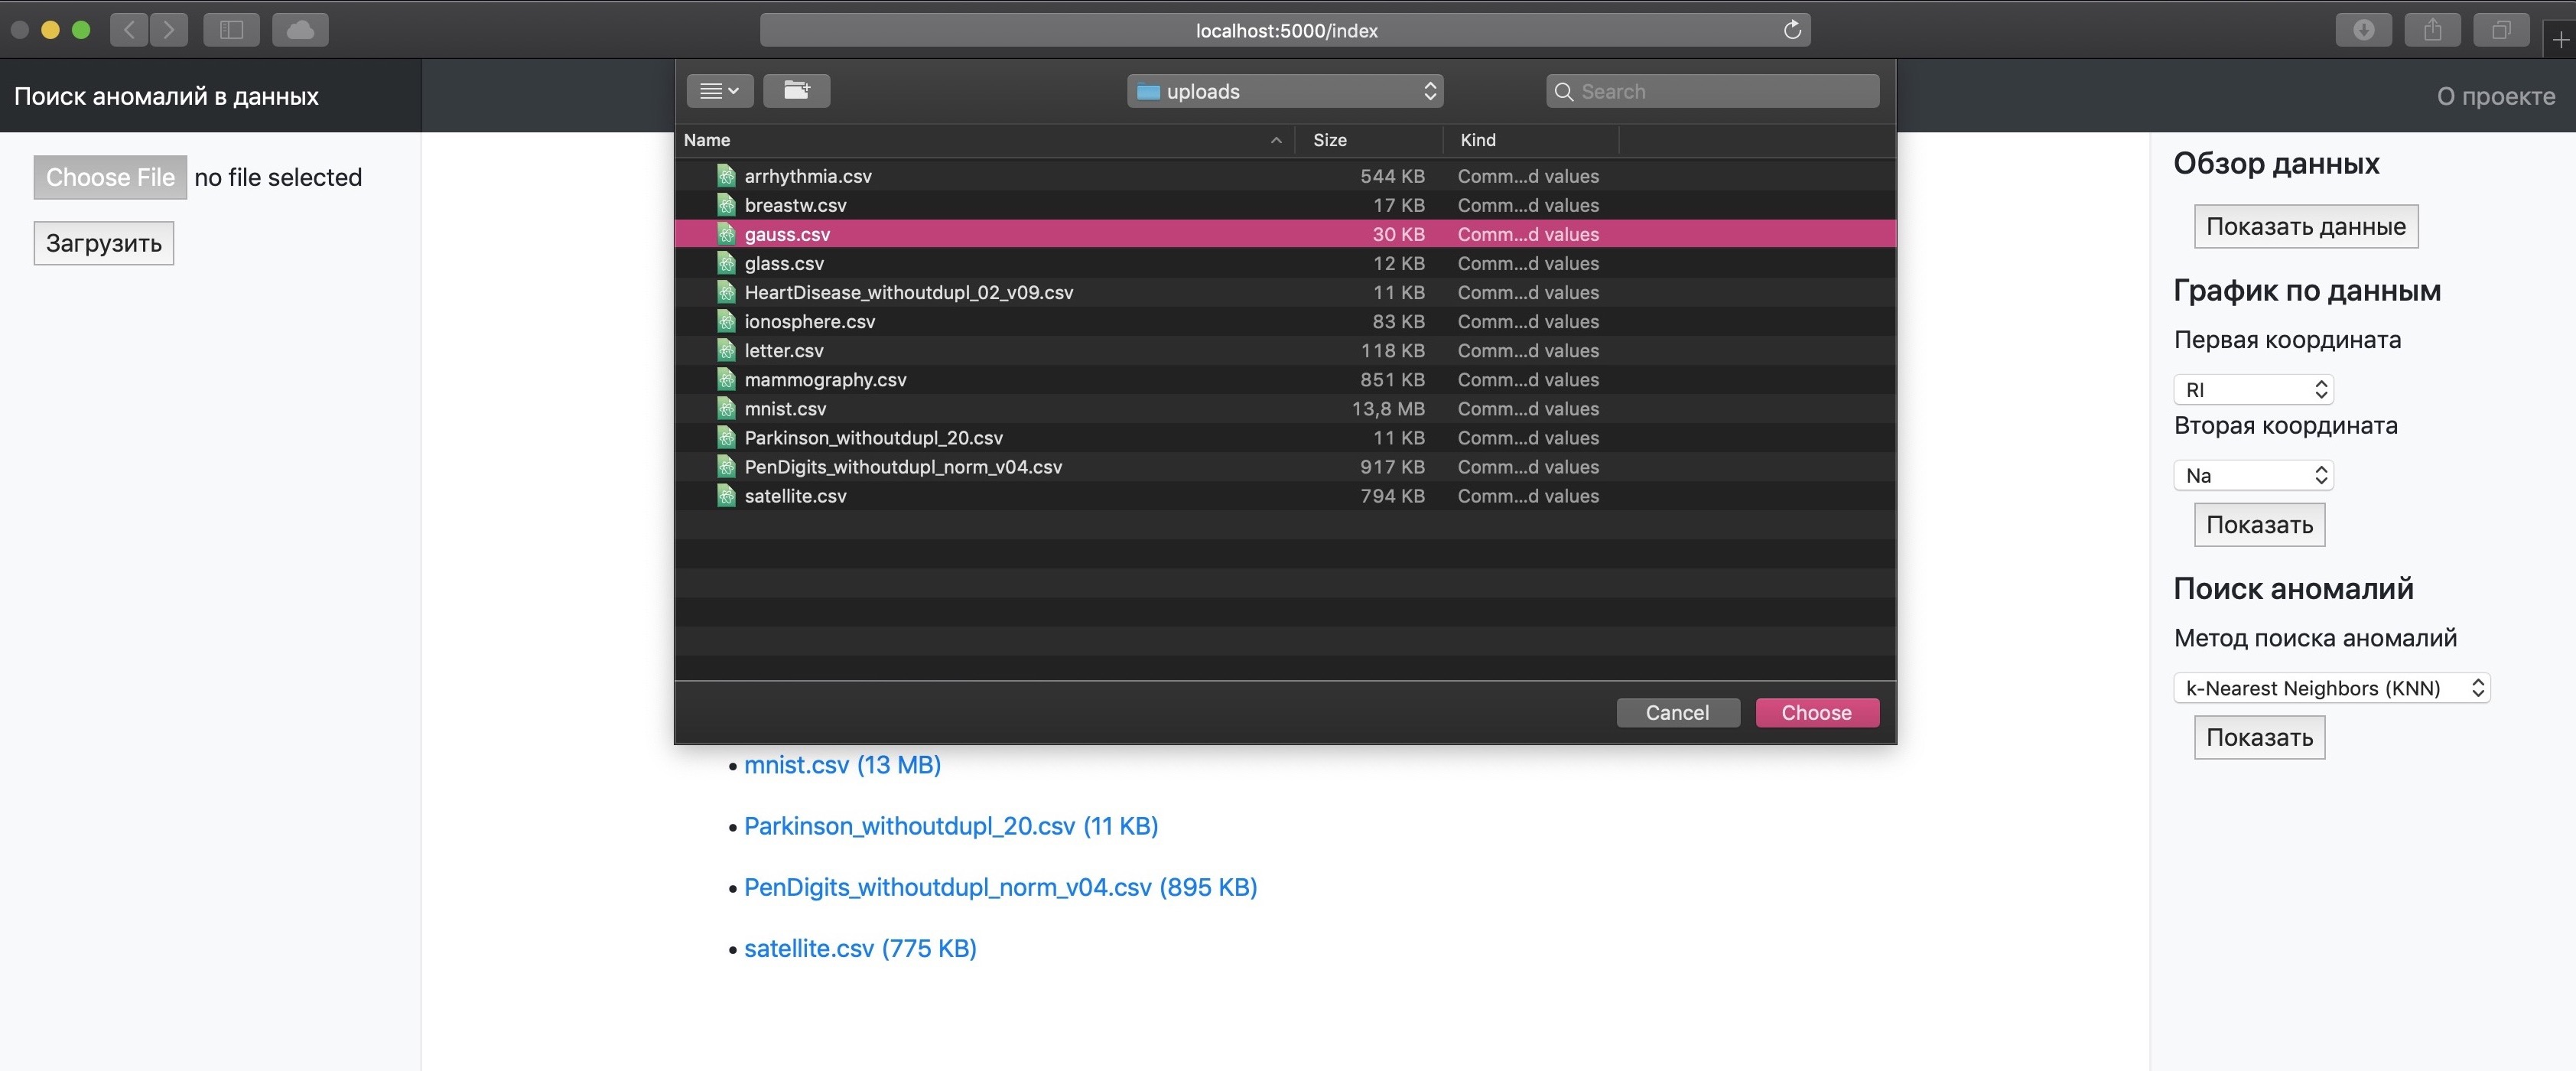
\includegraphics[width=\textwidth, height=\textheight, keepaspectratio] {demo_uploadfile}
  \caption{Пример экрана загрузки набора данных на сервер.}
  \label{fig:demo_uploadfile}
\end{figure}

\begin{figure}[ht]
  \centering
  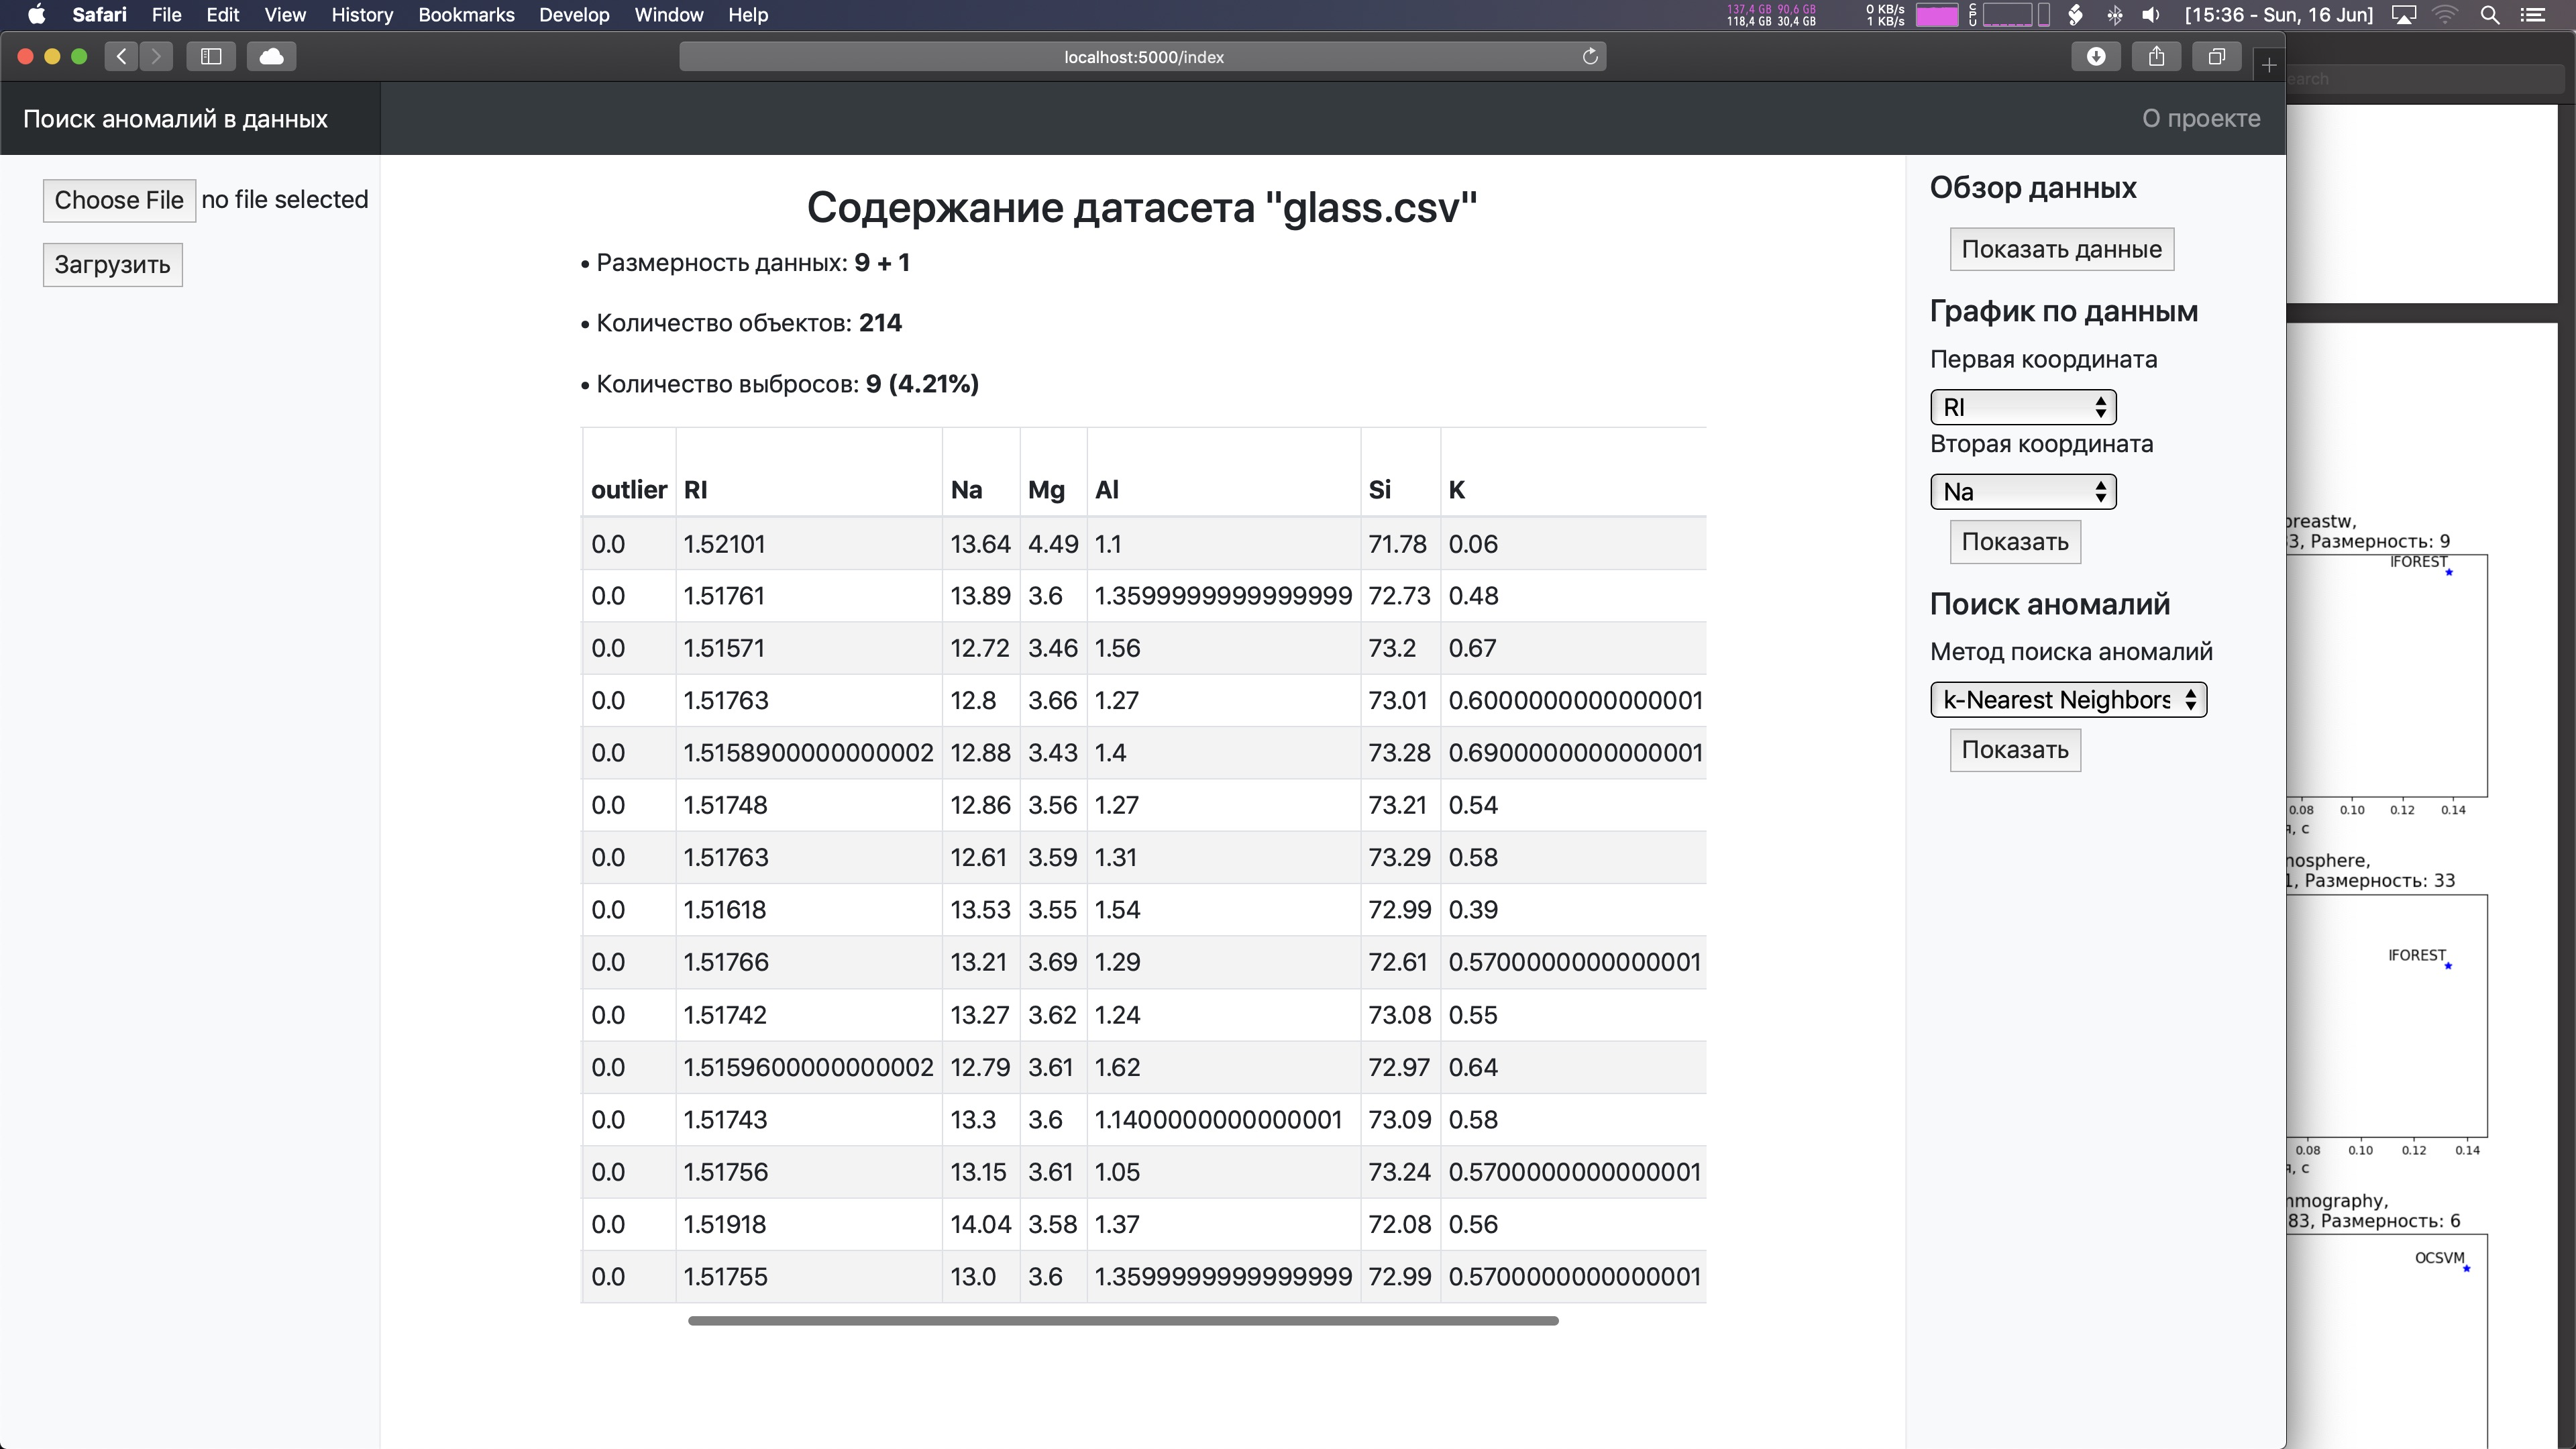
\includegraphics[width=\textwidth, height=\textheight, keepaspectratio] {demo_datasetloaded}
  \caption{После выбора файла на экране появляется таблица с некоторыми объектами из указанного набора данных. С помощью меню, которое располагается справа, можно выбрать: (\textbf{i}) построение общего графика по набору данных, на котором будут представлены данные, размерность которых была понижена с помощью метода t-SNE (продемонстрировано на рисунке~\ref{fig:demo_datasetoverview}), \textbf{(ii)} график зависимости одной из размерностей данных от другой (продемонстрировано на рисунке~\ref{fig:demo_plots}) и (\textbf{iii}) выбрать алгоритм из списка, с помощью которого будет осуществлён поиск аномалий в данных (продемонстрировано на рисунке~\ref{fig:demo_anomalydetection}).}
  \label{fig:demo_datasetloaded}
\end{figure}

\clearpage

\section{Основные функции}

\begin{figure}[ht]
  \centering
  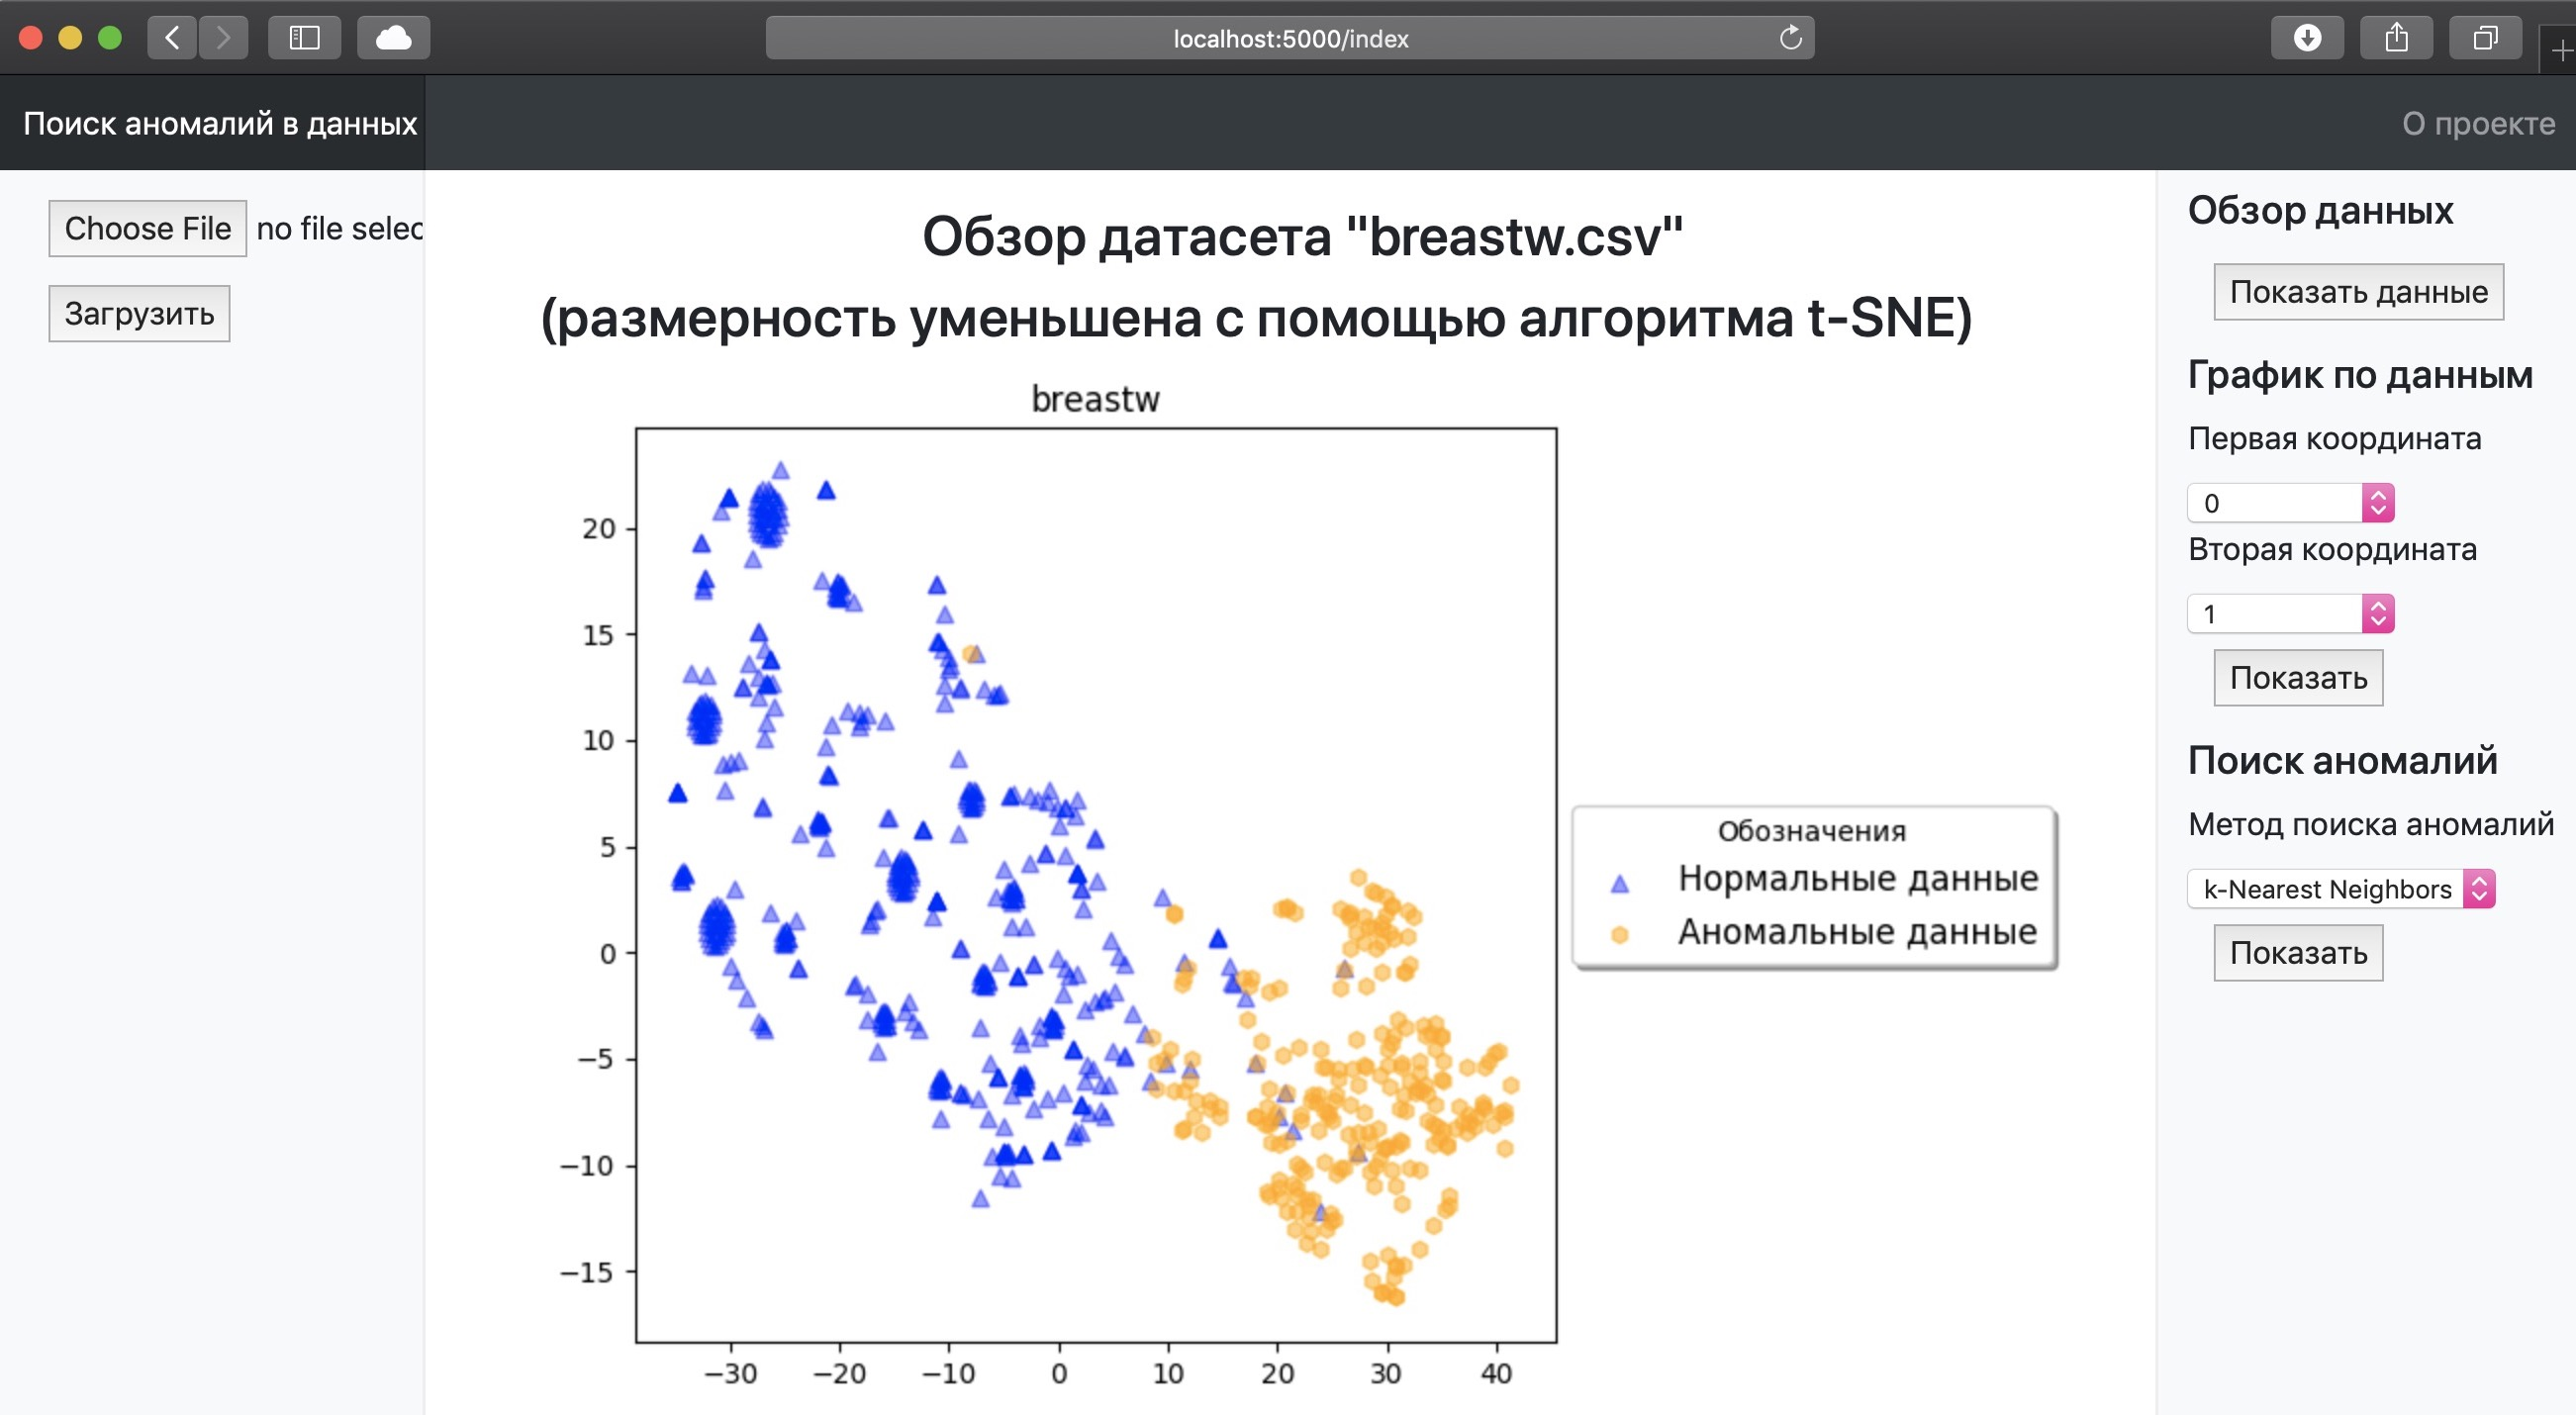
\includegraphics[width=\textwidth, height=\textheight, keepaspectratio] {demo_datasetoverview}
  \caption{Представление данных после понижения размерности до dim=2 при помощи алгоритма t-SNE.}
  \label{fig:demo_datasetoverview}
\end{figure}

\begin{figure}[ht]
  \centering
  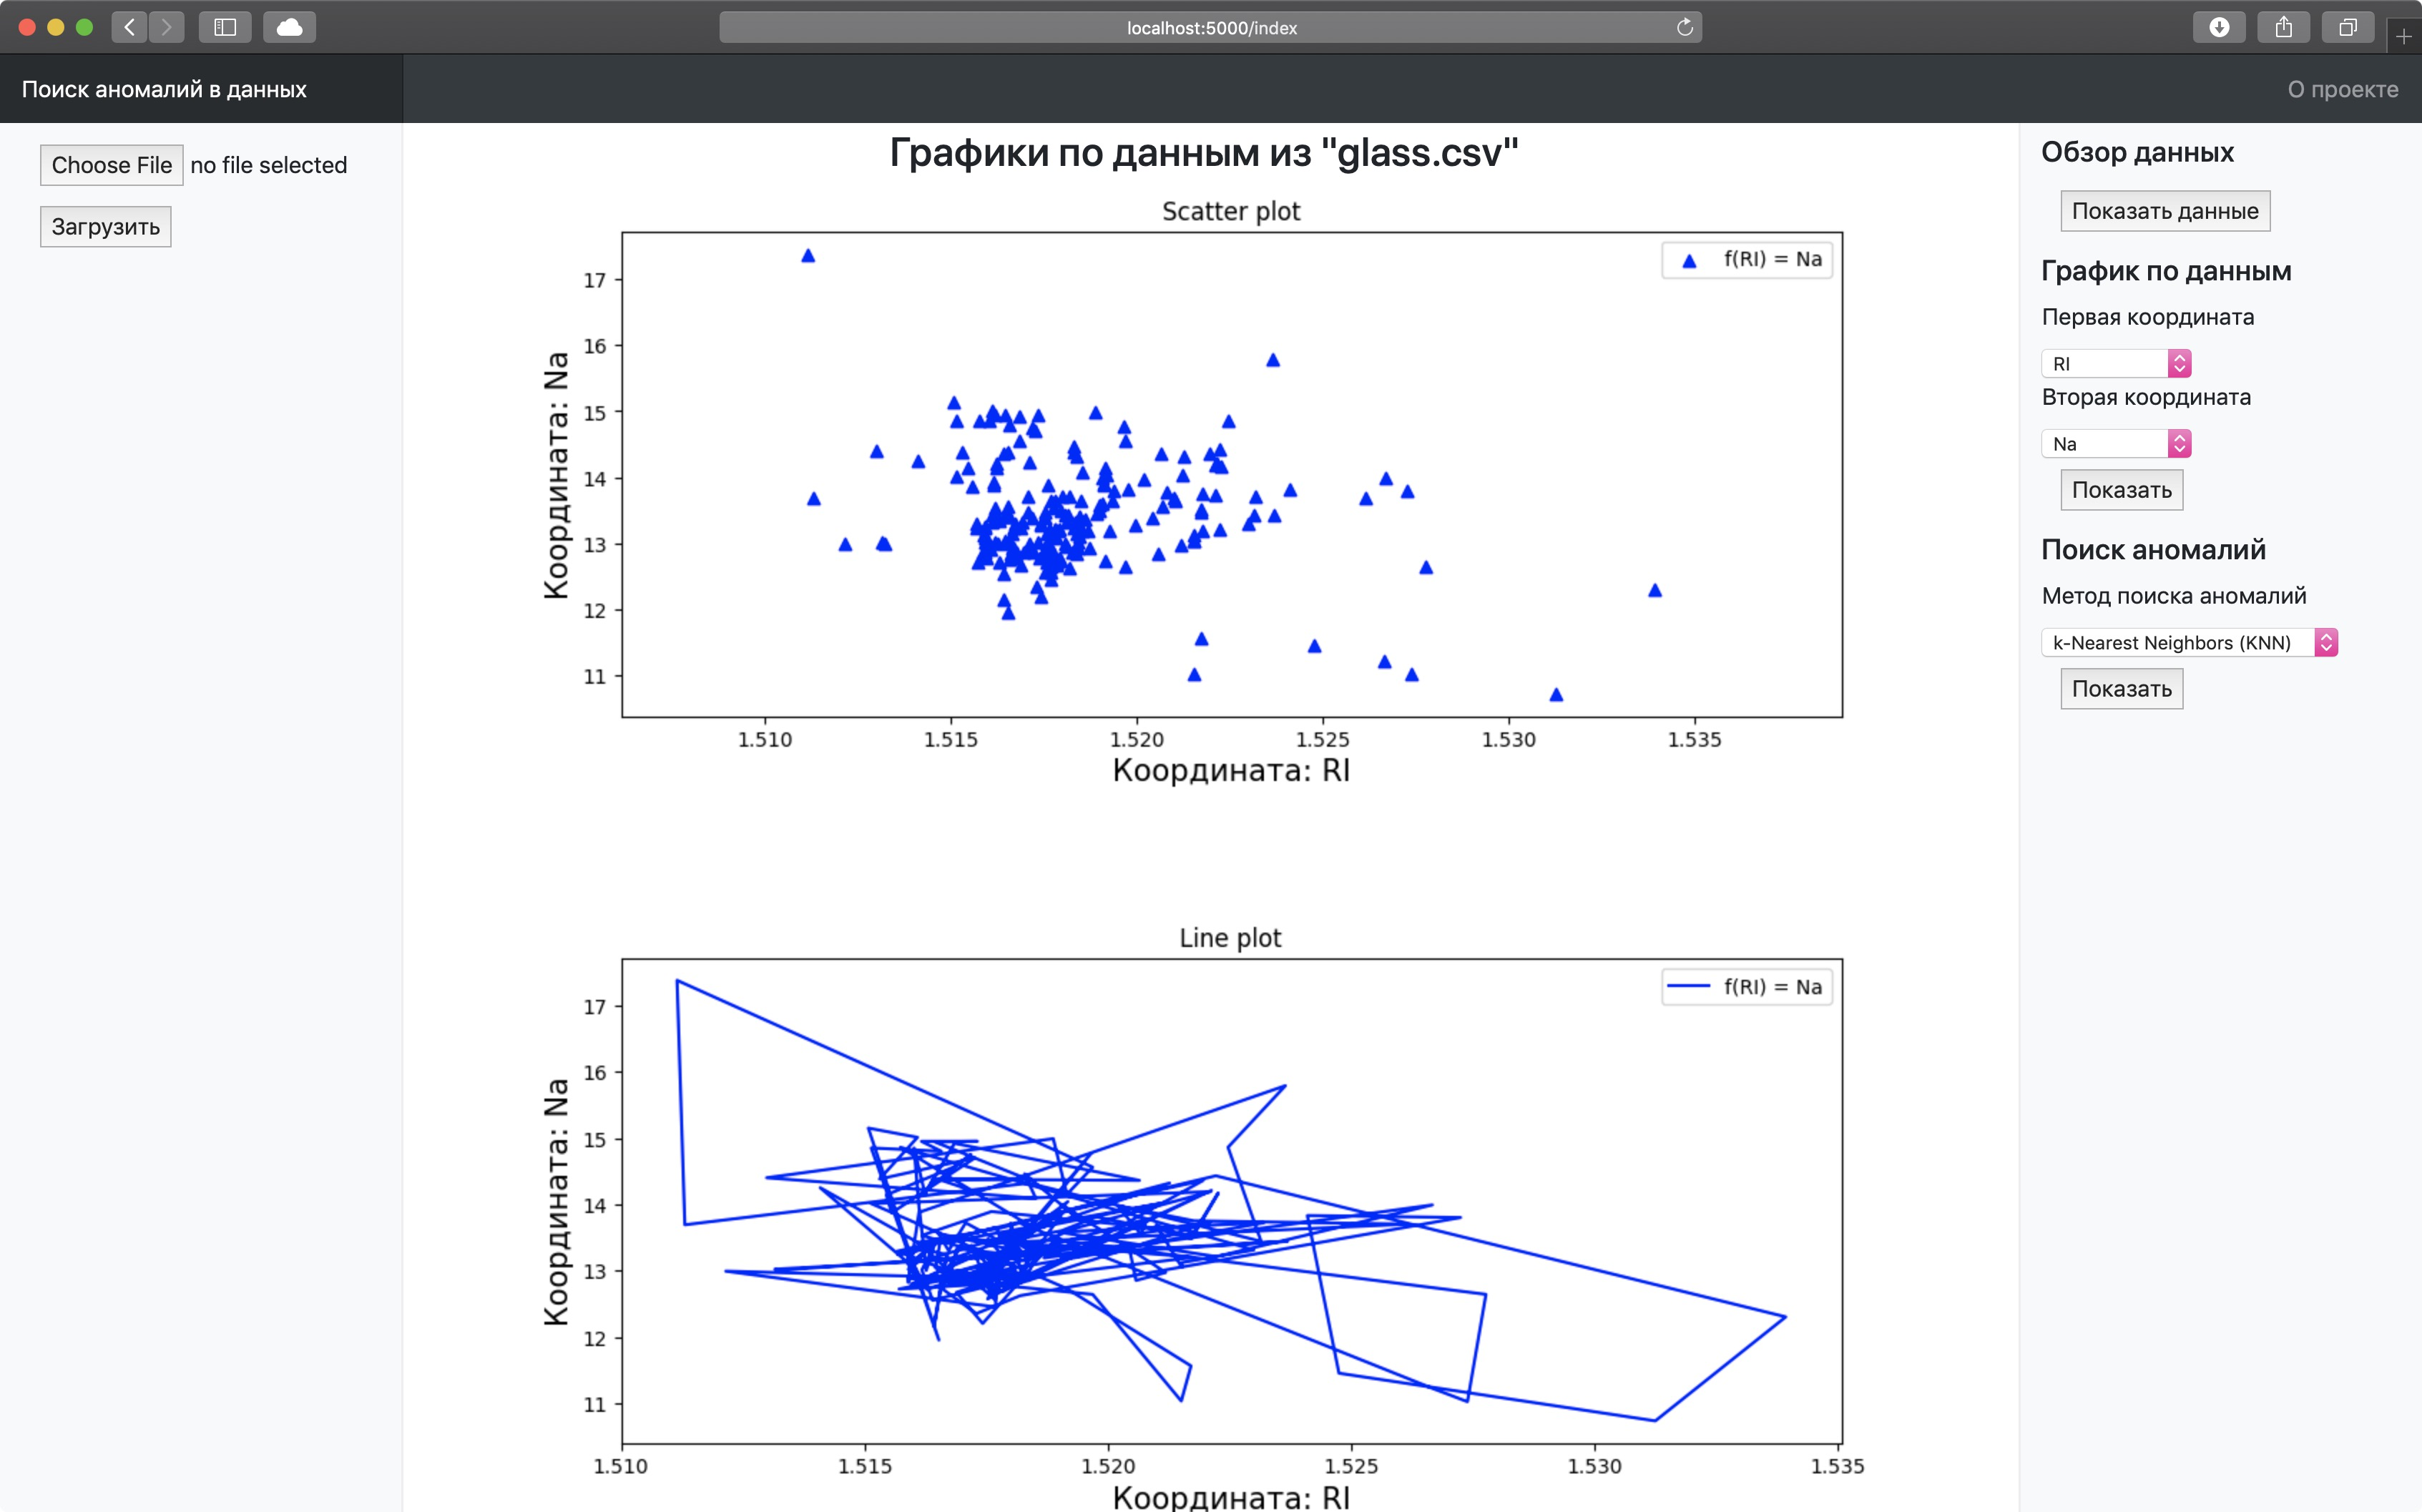
\includegraphics[width=\textwidth, height=\textheight, keepaspectratio] {demo_plots}
  \caption{Построение графика зависимости для указанных координат. На рисунке представлена зависимость максимального количества ударов в минуту от возраста пациентов (данные из датасета сердечных заболеваний).}
  \label{fig:demo_plots}
\end{figure}

\begin{figure}[ht]
  \centering
  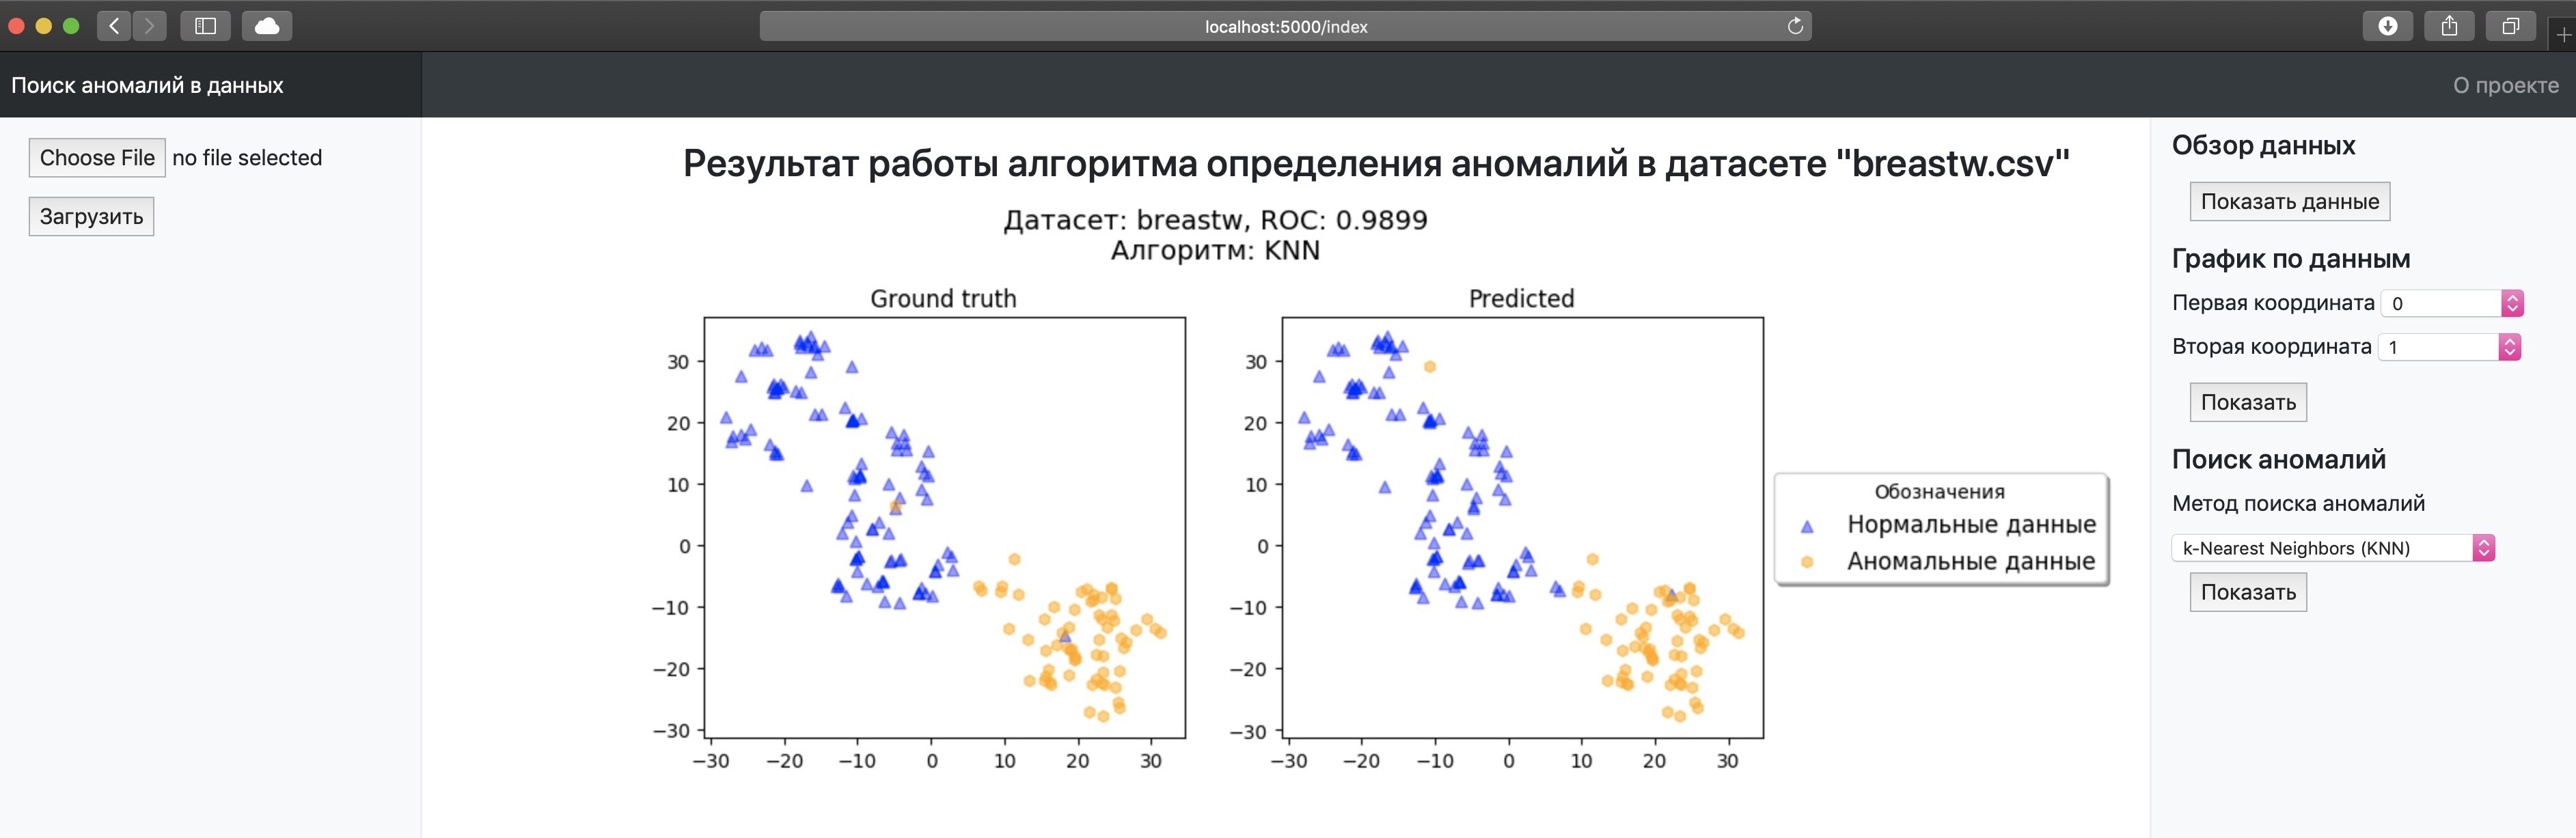
\includegraphics[width=\textwidth, height=\textheight, keepaspectratio] {demo_anomalydetection}
  \caption{Поиск аномалий в данных. Набор данных разбивается на две непересекающиеся части: на первой части выбранная модель обучается, а на второй -- проверяется качество обученной модели. Обычно, разделение происходит в соотношении 75\% и 25\% соответственно. Так снижается вероятность переобучения на данных, что позволяет избежать ухудшения обобщающей способности алгоритма.}
  \label{fig:demo_anomalydetection}
\end{figure}

\clearpage